\chapter{Conclusiones}
\label{chap:conclusiones}

\section{Resultados obtenidos}
En esta sección se presenta una vista global de los resultados obtenidos tras el ciclo de desarrollo, evaluando el grado de cumplimiento de las metas propuestas inicialmente, destacando los hitos tecnológicos alcanzados y documentando aquellos requisitos que han sido pospuestos.

\subsection{Requisitos funcionales}
En relación con el alcance funcional definido en las fases de análisis, se ha logrado implementar satisfactoriamente la inmensa mayoría de los requisitos priorizados. El desarrollo ha culminado con éxito en la materialización de los dos pilares fundamentales y diferenciadores del sistema:

\begin{itemize}
    \item \textbf{Visualización interactiva e intuitiva:} Se ha construido con éxito el Árbol de Trabajo (\emph{Tree View}), logrando abstraer la complejidad jerárquica de un proyecto en un grafo interactivo. Esta funcionalidad cumple el objetivo de permitir a los gestores y desarrolladores comprender el progreso y las dependencias de las tareas mediante una interfaz que minimiza la carga cognitiva frente a las herramientas tradicionales.
    \item \textbf{Orquestación de agentes autónomos:} Se ha implementado un motor de ejecución de agentes de \ac{IA} funcional. El sistema es capaz de instanciar agentes que actúan como miembros proactivos del equipo, reaccionando a eventos del dominio, interactuando con el sistema de forma autónoma y comunicándose de manera natural mediante el módulo de chats integrado.
\end{itemize}

No obstante, la gestión ágil del alcance temporal obligó a realizar ajustes pragmáticos durante los últimos \emph{sprints}. La \textbf{Épica de Perfil (Historias de Usuario 28 a 32)} no ha sido implementada en esta primera versión del producto. Esta épica contemplaba la generación de un perfil avanzado para cada usuario, incorporando métricas de productividad, calidad técnica, experiencia y sesgos de estimación. 

Al tratarse de funcionalidades de mejora continua (clasificadas mayoritariamente como \emph{Could Have} mediante el método MoSCoW), se tomó la decisión técnica de descartar su desarrollo para priorizar la estabilidad y la calidad de los módulos del camino crítico. En consecuencia, este bloque funcional queda perfectamente documentado y perfilado como una línea de desarrollo futuro, especialmente para enriquecer el contexto algorítmico que consumen los agentes de IA al asignar tareas.

\subsection{Requisitos no funcionales}
La evaluación de los atributos de calidad y restricciones globales del sistema revela un alto grado de cumplimiento, validando las decisiones arquitectónicas adoptadas durante las fases de diseño. A continuación, se detalla el estado final de los principales requisitos no funcionales:

\begin{itemize}
    \item \textbf{Mantenibilidad y Calidad del Código:} Este ha sido uno de los aspectos más exitosos del proyecto. Se ha implementado una arquitectura con una estricta separación de responsabilidades. Además, se ha superado holgadamente el requisito inicial del 80\% de cobertura, alcanzando más de un \textbf{90\% de cobertura de lineas} en las capas críticas del \emph{backend} (Dominio y Aplicación). Esto blinda la lógica de negocio frente a cambios, queda evidenciado en el reporte de cobertura de la solución (ver Figura \ref{fig:test_coverage}).
    
    \item \textbf{Seguridad y Control de Acceso:} Se ha cumplido el objetivo de implementar una autenticación estandarizada sin almacenar estado en el servidor. La integración con Google, respaldada por la emisión de \ac{JWT} en memoria y \emph{Refresh Tokens} rotatorios en \emph{cookies} \texttt{HttpOnly}, blinda la plataforma contra vectores de ataque comunes como \ac{XSS} o \ac{CSRF}. Asimismo, el modelo de autorización basado en roles (RBAC) opera de forma granular gracias a la intercepción de comandos mediante el patrón \emph{Decorator}.
    
    \item \textbf{Rendimiento y Tiempos de Respuesta:} Para validar las métricas de latencia, se ejecutaron baterías de pruebas de carga automatizadas utilizando \texttt{k6} para simular la carga. Las simulaciones confirmaron que, bajo condiciones de carga estándar (unos 30 usuarios), el percentil 95 de las peticiones síncronas se mantiene muy por debajo del umbral objetivo de los 300ms (ver Figura \ref{fig:performance}). Paralelamente, la delegación de tareas pesadas a procesos asíncronos en segundo plano (\emph{Background Jobs}) ha garantizado que el hilo principal nunca se bloquee.
    
    \item \textbf{Escalabilidad y Disponibilidad:} Al estar la infraestructura de despliegue alojada en los servicios de Microsoft Azure (mediante el programa \emph{Azure for Students}), el sistema hereda directamente los \ac{SLA} del proveedor \emph{cloud}. En concreto, el \ac{SLA} de Microsoft para máquinas virtuales de instancia única con SSD Premium garantiza un \emph{uptime} del \textbf{99,9\%} \cite{azure_sla_vm}, cumpliendo con el requisito de disponibilidad exigido. La escalabilidad horizontal queda teóricamente garantizada gracias a la contenerización con Docker y a la naturaleza \emph{stateless} del servidor web.
    
    \item \textbf{Usabilidad y Fluidez Visual:} El renderizado del Árbol de Trabajo en el cliente de React ha demostrado mantener la tasa de fotogramas requerida, permitiendo manipulaciones fluidas del grafo de tareas incluso con conjuntos de datos densos. La adopción del sistema de diseño \emph{shadcn/ui} ha asegurado el cumplimiento de las heurísticas de Nielsen y las directrices de contraste de accesibilidad web \cite{w3c2018wcag21}.
\end{itemize}

\begin{figure}[htbp]
    \centering
    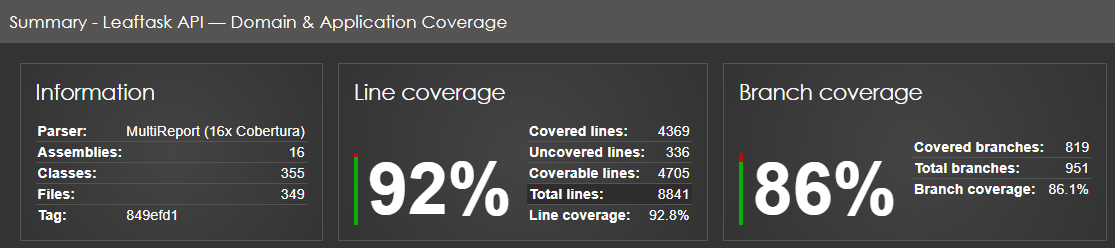
\includegraphics[width=0.9\textwidth]{images/content/Conclusiones/coverage-report.png}
    \caption{Reporte de cobertura de código.}
    \label{fig:test_coverage}
\end{figure}

\begin{figure}[htbp]
    \centering
    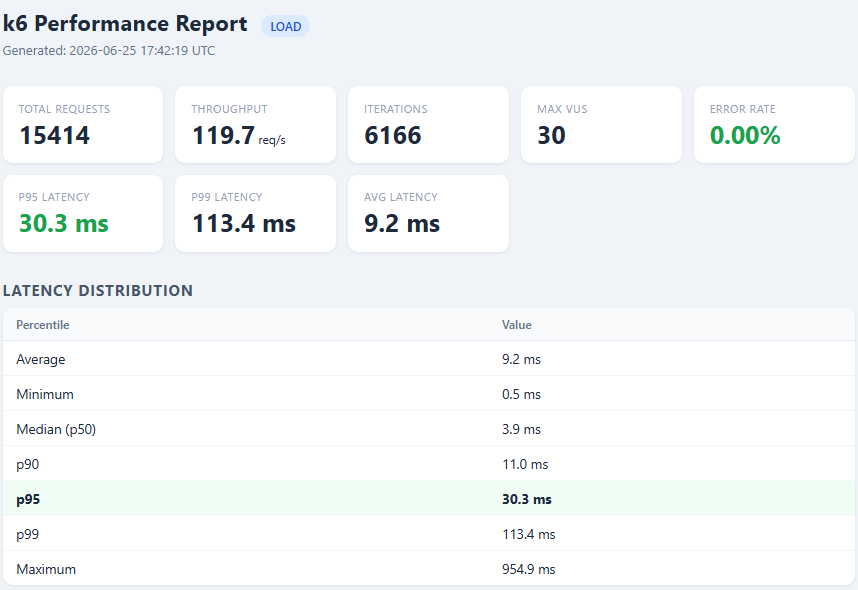
\includegraphics[width=0.9\textwidth]{images/content/Conclusiones/performance.png}
    \caption{Resultados de la prueba de carga}
    \label{fig:performance}
\end{figure}